\documentclass[11pt]{article}

% "review" for ARR submission (anonymous, line numbers); "final" for camera-ready; "preprint" for arXiv.
\usepackage[review]{acl}

\usepackage{times}
\usepackage{latexsym}
\usepackage[T1]{fontenc}
\usepackage[utf8]{inputenc}
\usepackage{microtype}
\IfFileExists{inconsolata.sty}{\usepackage{inconsolata}}{}
\usepackage{graphicx}
\usepackage{booktabs}
\usepackage{amsmath}
\usepackage{xcolor}
\usepackage{multirow}

% Cells that wait for the open-weight runs; make_acl.py writes the numbers once every run is present.
\newcommand{\pend}{\textcolor{red}{pending}}
\newcommand{\todo}[1]{\textcolor{red}{[#1]}}

\title{When the Answer Key Shares the Tool's Bug: Evaluating Tool-Augmented\\Language Models on Rare-Disease Clinical-Development Questions}

\author{Anonymous ACL submission}

\begin{document}
\maketitle

\begin{abstract}
Benchmarks for tool-using language models usually derive their gold answers from the same sources the tools query. We show that this can hide errors. We release RareMCP, read-only Model Context Protocol (MCP) servers over six public biomedical sources, and 314 clinical-development questions about rare and neglected tropical diseases (NTDs) with gold answers computed from raw source responses. We compare four tool conditions (no tools, web search, an existing biomedical MCP server, and RareMCP) for two closed and two open-weight models. As expected for questions drawn from the wrapped sources, RareMCP was the most accurate condition on single-source questions (96.5--99.2\% for the closed models). More instructive, a Drugs@FDA search bug shared by RareMCP and the gold-answer code made the tool look perfect on one template (100\%) until an independent re-derivation dropped it to 58\%. Web search failed mostly because it could not reach structured data, not because pages were stale, and was weakest on NTDs. Without tools, one model narrated tool calls that never ran. \todo{One sentence on the open-weight results once the runs finish.}
\end{abstract}

\section{Introduction}

Teams developing treatments for rare diseases and neglected tropical diseases (NTDs) look up facts that are spread across public resources: trial status and enrolment in ClinicalTrials.gov \citep{ctgov}, target--disease evidence and the drugs tested for a disease in Open Targets \citep{opentargets}, approval history in ChEMBL \citep{chembl}, generic availability and boxed warnings in Drugs@FDA and FDA labels \citep{openfda}, and prevalence, which decides rarity under the EU definition \citep{eurare}, in Orphanet \citep{orphadata}. These teams are often small and investigator-led, and many rare-disease trials are never completed or published \citep{rees2019}. Language models answer such questions fluently from parametric memory, but that memory is dated by construction and weakest for rarely mentioned entities \citep{kandpal2023}, and models state unsupported facts confidently \citep{ji2023}. Tool use is the standard remedy \citep{toolformer, genegpt}, and the Model Context Protocol (MCP) now gives a common interface through which any compatible client can call such tools \citep{mcp}.

How should these tools be evaluated? The convenient design, used by ToolQA \citep{toolqa} and by most single-resource MCP studies \citep{m3, disphasedb, ehrmcp}, generates questions from the data a tool exposes and computes gold answers from that same data. The design is scalable and reproducible, but it gives the tool and the answer key a common path to the source. If both take the same wrong turn, the tool will agree with the wrong answer and be scored correct. Errors in gold labels are known to distort benchmark rankings \citep{northcutt2021, gema2025}; the specific risk here is that the error is \emph{correlated} with the system under test.

We report a case where this happened, in a controlled evaluation that we would otherwise have published as a clean win for our tool. Our contributions are:
\begin{itemize}
\setlength\itemsep{0pt}
\item \textbf{A resource:} RareMCP, six read-only MCP servers over public sources in which every response carries provenance, and 314 questions from 18 templates (254 single-source, 60 multi-step), with gold answers, audit payloads and the logs of every run (\S\ref{sec:resource}).
\item \textbf{A benchmark-validity finding:} a Drugs@FDA search error shared by the tool and the gold-answer code inflated the tool's accuracy until an independent re-derivation found it (\S\ref{sec:shared}).
\item \textbf{A controlled comparison} of no tools, web search, BioMCP \citep{biomcp} and RareMCP for two closed models (Claude Sonnet 5.5 and Haiku 5.5) and two open-weight models (Gemma 4 26B-A4B and gpt-oss-20b), showing where general web search and a general biomedical MCP server fall short and why (\S\ref{sec:results}).
\item \textbf{An error mode:} models without tools sometimes narrate tool calls and results that never happened (\S\ref{sec:fab}).
\end{itemize}
RareMCP's near-perfect accuracy on single-source questions is the expected outcome of this design and is not what we consider the contribution.

\section{Related work}

\paragraph{Tool-use benchmarks.} API-Bank \citep{apibank}, ToolLLM \citep{toolllm} and BFCL \citep{bfcl} test whether models choose and call functions correctly, often scoring the call rather than the answer. ToolQA \citep{toolqa} scores answers to questions generated from external corpora that the tools access, the design we adopt; it was built to separate tool use from memorisation, and our results show a cost of that design that, to our knowledge, has not been reported: gold-answer code and tools can fail together.

\paragraph{Biomedical tools for language models.} GeneGPT taught a model to call NCBI web APIs and raised accuracy on genomics questions well above retrieval-free baselines \citep{genegpt}; TrialGPT uses models over trial records for patient matching \citep{trialgpt}. Published MCP evaluations in biomedicine address single resources, such as an intensive-care database \citep{m3}, a protein-variant database \citep{disphasedb} and a hospital record system \citep{ehrmcp}, and usually compare against unaided models. Open biomedical MCP servers exist, notably BioMCP \citep{biomcp}. We are not aware of a controlled comparison spanning trial, target, drug and prevalence sources against both web search and another biomedical MCP server.

\paragraph{Gold-label errors.} Label errors in test sets can reorder model rankings \citep{northcutt2021}, and a substantial share of MMLU questions have wrong or ambiguous answers \citep{gema2025}. Those errors come from human annotation and are not tied to any one system. The error we describe is generated by code and correlated with the system under test, so it inflates exactly the model it should evaluate.

\section{RareMCP and the question set}
\label{sec:resource}

\paragraph{Servers.} RareMCP is six Python MCP servers, one per source, plus a combined server, over ClinicalTrials.gov, Open Targets, ChEMBL, openFDA, Europe PMC \citep{europepmc} and Orphadata, with 17 read-only tools in total (trial search and retrieval; disease targets and drugs; molecule look-up, mechanisms and indications; Drugs@FDA generic availability and labels; literature search; disorder prevalence with an EU-rarity classification). Every tool returns the same envelope: data, total, a next-page token, notes and a provenance list giving the source URL, data release and retrieval time. The HTTP layer throttles each host, retries transient failures and can record and replay responses, so runs are reproducible offline. It is unrelated to BioMCP.

\paragraph{Questions.} Seeded scripts generated 314 questions from 18 templates (Appendix~\ref{app:templates}). From the 5,446 Orphanet disorders with an exact, validated MONDO cross-reference, 4,014 were rare under the EU definition with at least medium-confidence prevalence; we drew 160 at random and added 24 WHO-listed NTDs \citep{who_ntd} that resolved to Open Targets diseases. A balanced rarity template drew 10 rare and 10 non-rare disorders, and 20 questions name trial or compound identifiers confirmed not to exist (HTTP 404), to test abstention. Base-tier questions (254) are answerable from one source; hard-tier questions (60) need several steps or sources. Forty-eight questions concern NTDs and 246 rare diseases.

\paragraph{Gold answers.} Gold answers were computed on 3--4 November 2026 from raw API responses by deterministic code that does not import the servers; each question stores its source URLs and retrieval time. Scoring rules depend on answer type: exact match for yes/no, years and integers; tolerances for counts; set F1 against the gold set (threshold 0.5--0.6); token F1 for free text; and abstention for non-existent identifiers.

\paragraph{Audit.} We re-fetched the primary record for a stratified sample of 41 questions and re-derived answers with separately written code; all 41 matched. Prompted by one item flagged in question screening, we then re-derived every Drugs@FDA-dependent answer (58 questions) by a \emph{different query path}, the union of the openFDA generic-name and active-ingredient searches. Eight gold answers changed (\S\ref{sec:shared}); the corrected set (v1.1) is used throughout.

\paragraph{Expert review.} Three raters scored all 314 questions from 1 to 5 for clinical relevance, realism and gold-answer correctness: a clinical pharmacologist with 10 years' NHS experience, a consultant epidemiologist and one of the authors, a clinician who designed the questions. With scores grouped as low (1--2), moderate (3) or high (4--5) and pooled over dimensions, Fleiss' $\kappa$ was 0.78. No question was dropped or edited because of the ratings.

\section{Experimental setup}
\label{sec:setup}

\paragraph{Conditions.} Each question was put to each model once under four conditions: \emph{no tools}; \emph{web search}; \emph{BioMCP} (GenomOncology's open server, biomcp-cli 0.9.3, covering trials, literature, variants, Open Targets, ChEMBL and openFDA); and \emph{RareMCP}. Conditions with MCP servers had no web access. All conditions shared one system prompt, written before the main runs and not tuned on results, asking for a final JSON block with the answer, the identifiers relied on, a not-found flag and a confidence in $[0,1]$, and telling the model never to invent identifiers. Runs were capped at 20 turns.

\paragraph{Closed models.} Claude Sonnet 5.5 and Claude Haiku 5.5 (reliable knowledge cut-off June 2026; \citealp{claude55}) ran through headless Claude Code \citep{claudecode} with default sampling, a 600-s timeout and only the condition's tools enabled; web search used Claude Code's built-in WebSearch and WebFetch. The 2,512 runs took place 3--10 November 2026 with RareMCP 0.1.0. Under Claude Code the BioMCP server closed its connection about 5~s after each client session; we therefore re-ran the whole BioMCP condition behind a pass-through proxy that holds one session and forwards tool lists, calls and results unchanged, and report those runs. Attempts ended by a usage limit or other infrastructure error (172) were re-run.

\paragraph{Open-weight models.} Gemma 4 26B-A4B (a mixture-of-experts model with 3.8B active parameters; training cut-off January 2025; \citealp{gemma4}) and gpt-oss-20b (\citealp{gptoss}; cut-off June 2024), both Apache-2.0, were served with llama.cpp \citep{llamacpp} on CPU-only, GitHub-hosted runners, using quantised weights (Gemma QAT Q4\_0; gpt-oss MXFP4) pinned by repository revision, a 32,768-token context and each developer's recommended sampling. A small client sent the same system prompt, questions and turn cap through the OpenAI-compatible chat API with native tool calling, with a 1,200-s timeout and tool outputs truncated to 12,000 characters to fit the context. Running out of turns, time or context counted as an incorrect answer. A turn that ended with no text, or with a tool call written as plain text that the server could not parse (both models did this without tools), received one reply asking for the final answer, as Claude Code replies to a call for a tool it does not have; we report how often this happened. RareMCP and BioMCP were attached over stdio (no proxy was needed). For web search, these models had a DuckDuckGo search tool and a fetch tool returning page text: the same purpose as Claude Code's tools, not the same implementation. They used RareMCP 0.1.1, which contains the corrected Drugs@FDA search. These runs used no paid service: weights, server, search and runners were free, and the client refuses any non-local model endpoint.

\paragraph{Outcomes and statistics.} The primary outcome is accuracy against gold v1.1 on all questions. Secondary outcomes are identifier validity (every NCT, ChEMBL and PubMed identifier checked against the live source), grounding (cited identifiers present in the run's tool outputs), expected calibration error over 10 bins \citep{guo2017} and Brier score \citep{brier1950}. We report Wilson 95\% intervals \citep{wilson1927}, compare RareMCP with each comparator within model on identical questions using the exact McNemar test \citep{mcnemar1947} with a question-level paired bootstrap interval (10,000 resamples; \citealp{efron1993}), and use $\alpha=0.05$ without multiplicity correction. Analyses added after the first results are labelled post hoc.

\section{Results}
\label{sec:results}

\begin{figure*}[t]
\centering
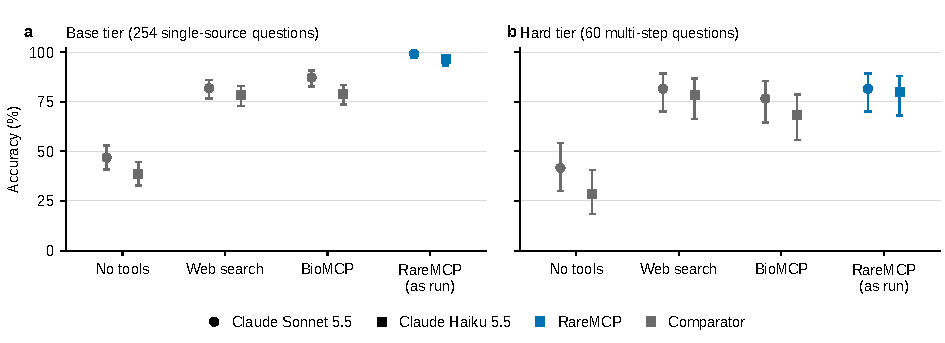
\includegraphics[width=\textwidth]{fig_accuracy.pdf}
\caption{Accuracy by tool condition (gold v1.1), one run per question, model and condition, with Wilson 95\% intervals. Blue: RareMCP as run (0.1.0 for the Claude models, 0.1.1 for open-weight models); grey: comparators. Filled markers: closed models; hollow markers: open-weight models.}
\label{fig:acc}
\end{figure*}

\begin{table*}[t]
\centering\small
\begin{tabular}{llccccc}
\toprule
Tier & Model & No tools & Web search & BioMCP & RareMCP 0.1.0 & RareMCP 0.1.1 \\
\midrule
Base & Claude Sonnet 5.5 & 46.9 & 81.9 & 87.4 & \textbf{99.2} & 100.0$^\dagger$ \\
Base & Claude Haiku 5.5 & 38.6 & 78.3 & 79.1 & \textbf{96.5} & 97.2$^\dagger$ \\
Base & Gemma 4 26B-A4B & \pend & \pend & \pend & -- & \pend \\
Base & gpt-oss-20b & \pend & \pend & \pend & -- & \pend \\
\midrule
Hard & Claude Sonnet 5.5 & 41.7 & 81.7 & 76.7 & \textbf{81.7} & 90.0$^\dagger$ \\
Hard & Claude Haiku 5.5 & 28.3 & 78.3 & 68.3 & \textbf{80.0} & 90.0$^\dagger$ \\
Hard & Gemma 4 26B-A4B & \pend & \pend & \pend & -- & \pend \\
Hard & gpt-oss-20b & \pend & \pend & \pend & -- & \pend \\
\bottomrule
\end{tabular}
\caption{Accuracy (\%) by tool condition against the audited gold answers (v1.1), one run per question, model and condition. Base tier: 254 single-source questions; hard tier: 60 multi-step questions. Bold: RareMCP version as run. Claude models were run with RareMCP 0.1.0; $^\dagger$post hoc composite in which the 58 Drugs@FDA-dependent questions were re-run with 0.1.1 and all other answers kept (\S\ref{sec:shared}). Open-weight models were run once, with 0.1.1 throughout. Open-model web search is DuckDuckGo search plus page fetch rather than Claude Code's built-in tools (\S\ref{sec:setup}). 95\% Wilson intervals are in Figure~\ref{fig:acc}.}
\label{tab:acc}
\end{table*}


\subsection{Accuracy by condition}

On single-source questions, RareMCP was the most accurate condition for both closed models (Table~\ref{tab:acc}, Figure~\ref{fig:acc}): 99.2\% for Sonnet and 96.5\% for Haiku, against 81.9\% and 78.3\% with web search, 87.4\% and 79.1\% with BioMCP, and 46.9\% and 38.6\% without tools. It beat every comparator for both models ($P<2\times10^{-8}$; Table~\ref{tab:paired}). This is what a tool that queries the generating sources should do. On multi-step questions, RareMCP 0.1.0 only matched web search (Sonnet 81.7\% vs 81.7\%; Haiku 80.0\% vs 78.3\%) and did not differ significantly from BioMCP. In the tool conditions every answer parsed and no cited identifier was invalid; both MCP conditions were fully grounded (1,020 identifiers cited with RareMCP and 908 with BioMCP, all present in the run's tool outputs). RareMCP also had the lowest calibration error and Brier score, without increasing latency over web search (Appendix~\ref{app:calib}).

\begin{table}[t]
\centering
\setlength{\tabcolsep}{3pt}
\resizebox{\columnwidth}{!}{%
\begin{tabular}{llrrrr}
\toprule
& & \multicolumn{2}{c}{vs web search} & \multicolumn{2}{c}{vs BioMCP} \\
\cmidrule(lr){3-4}\cmidrule(lr){5-6}
Tier & Model & $\Delta$ & $P$ & $\Delta$ & $P$ \\
\midrule
Base & Sonnet 5.5 & +17.3 & $1.3\times10^{-12}$ & +11.8 & $1.5\times10^{-8}$ \\
Base & Haiku 5.5 & +18.1 & $1.0\times10^{-11}$ & +17.3 & $8.4\times10^{-12}$ \\
Base & Gemma 4 E4B & \pend & & \pend & \\
Base & gpt-oss-20b & \pend & & \pend & \\
\midrule
Hard & Sonnet 5.5 & +0.0 & 1.00 & +5.0 & 0.58 \\
Hard & Haiku 5.5 & +1.7 & 1.00 & +11.7 & 0.12 \\
Hard & Gemma 4 E4B & \pend & & \pend & \\
Hard & gpt-oss-20b & \pend & & \pend & \\
\bottomrule
\end{tabular}}
\caption{RareMCP minus comparator, accuracy in percentage points, paired on identical questions (gold v1.1); exact two-sided McNemar $P$. Claude: RareMCP 0.1.0 as run; open models: 0.1.1. Bootstrap intervals for every row are in Appendix~\ref{app:paired}.}
\label{tab:paired}
\end{table}


\subsection{A shared error between the tool and its answer key}
\label{sec:shared}

\begin{figure*}[t]
\centering
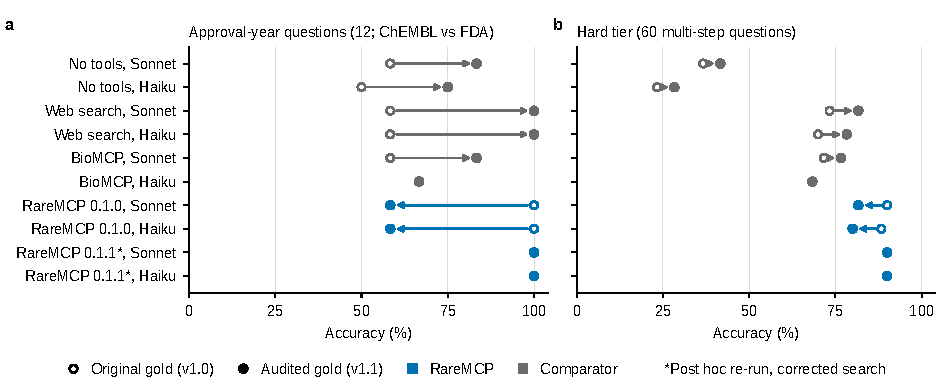
\includegraphics[width=\textwidth]{fig_shared_error.pdf}
\caption{Accuracy against the original (hollow) and audited (filled) gold answers for the Claude models; arrows show the change. (a) The 12 hard-tier questions asking whether ChEMBL's first-approval year matches the earliest FDA approval. (b) All 60 hard-tier questions. RareMCP 0.1.0 used the same incomplete Drugs@FDA search as the original gold code, so it agreed with the wrong answers and fell on correction while every comparator rose. *Post hoc re-run of the 58 Drugs@FDA-dependent questions with the corrected search, scored against v1.1 only.}
\label{fig:shared}
\end{figure*}

Searching Drugs@FDA by the openFDA generic-name field misses older applications that lack openFDA metadata; carboplatin's 1989 new drug application is one. The original gold code used that search, and so did RareMCP 0.1.0. Eight gold answers were wrong: 5 of the 12 approval-year questions, 2 generic-availability questions and 1 multi-step drug question.

Because the tool shared the error, it agreed with the wrong answers. On the approval-year template RareMCP scored 100\% for both models against the original gold and 58\% against the corrected gold, while web search, which reached FDA records by another route, rose from 58\% to 100\% (Figure~\ref{fig:shared}a). Against the original gold, RareMCP led web search on the hard tier by 16.7 points for Sonnet (90.0\% vs 73.3\%) and 18.3 points for Haiku (88.3\% vs 70.0\%); against the corrected gold the lead vanished (Figure~\ref{fig:shared}b). A re-derivation that reused the same search had matched all 41 audited items; only a different query path exposed the bug.

We fixed the search in RareMCP 0.1.1 and, post hoc, re-ran the 58 affected questions. With those answers substituted, accuracy was 100\% (Sonnet) and 97.2\% (Haiku) on the base tier and 90.0\% for both models on the hard tier; against web search on the hard tier the difference was $+8.3$ points for Sonnet (95\% CI $-1.7$ to 18.3; $P=0.18$) and $+11.7$ for Haiku (3.3 to 21.7; $P=0.039$).

\subsection{Where web search and BioMCP fell short}

\begin{table}[t]
\centering\footnotesize
\setlength{\tabcolsep}{3pt}
\resizebox{\columnwidth}{!}{%
\begin{tabular}{lcccc}
\toprule
Template & None & Web & BioMCP & RareMCP \\
\midrule
Top-5 targets & 15/5 & 10/0 & 85/85 & 100/100 \\
Drugs at phase $\geq$3 & 60/45 & 55/15 & 80/45 & 100/100 \\
EU rarity (chance 50) & 50/45 & 50/50 & 50/25 & 100/75 \\
Late-stage + generic & 57/50 & 57/64 & 71/57 & 100/100 \\
+ boxed warning (H) & 33/42 & 42/67 & 42/58 & 92/92 \\
Approval year (H) & 83/75 & 100/100 & 83/67 & 58/58 \\
Untested target drugs (H) & 75/8 & 67/33 & 58/17 & 58/58 \\
\bottomrule
\end{tabular}}
\caption{Accuracy (\%) for Sonnet/Haiku on the templates where conditions differed most (gold v1.1; RareMCP 0.1.0). H: hard tier. On single-trial facts printed on one ClinicalTrials.gov page, web search and RareMCP both scored 100\%.}
\label{tab:templates}
\end{table}

Web search matched RareMCP on facts printed on one ClinicalTrials.gov page (why a trial stopped, enrolment, whether an analysis plan was uploaded, number of sites: 100\% in both). The gaps opened where the answer is an aggregate or a ranking held in a structured resource (Table~\ref{tab:templates}). Without the Orphanet tool every condition scored at or below chance on EU rarity. BioMCP did well on Open Targets look-ups but has no prevalence tool, and 30\% of its tool calls returned an error from BioMCP itself, mostly requests for unsupported entities or sections. An MCP interface alone did not deliver the gain; coverage of the queries the task needs did.

\paragraph{Staleness or reach?} A natural objection is that web search was penalised for out-of-date pages. We classified all 125 incorrect web-search answers of the closed models by comparing the answer and the gold with the text the run retrieved. Forty-nine (39\%) were abstentions and 34 (27\%) involved data the run never retrieved, often after the model tried to call Open Targets' GraphQL interface, which a fetch tool cannot query. Only 12 (10\%) matched a retrieved source that disagreed with the database, the signature of stale pages; counting all 12 as correct would raise web-search base-tier accuracy by at most 1.6 points. Web search failed mainly because it could not reach the structured data.

\paragraph{NTDs.} The 48 NTD questions all come from aggregate templates. On them RareMCP answered 95.8\% correctly for both closed models, against 54.2\% (Sonnet) and 50.0\% (Haiku) with web search and 72.9\% and 68.8\% with BioMCP. On rare-disease questions from the same templates ($n=62$), web search scored 62.9\% and 48.4\% and RareMCP 93.5\% and 90.3\%. The subset is small and the analysis exploratory, but web search was weakest for the diseases with the least web coverage, while RareMCP was similar across populations.

\paragraph{Model size.} Without tools Haiku trailed Sonnet by 8.3 points on the base tier ($P=1.9\times10^{-4}$); with RareMCP the gap was 2.8 points, and Haiku gained 5.5 points more than Sonnet from RareMCP relative to no tools (95\% CI 0.8 to 10.2). With BioMCP the gap stayed at 8.3 points.

\subsection{Open-weight models}
\label{sec:open}

\textcolor{red}{[Open-weight runs pending; this paragraph and the open-model rows of Tables~\ref{tab:acc} and~\ref{tab:paired} are generated by \texttt{paper/acl/make\_acl.py} once every run is present.]}


\subsection{Fabricated tool use}
\label{sec:fab}

In the no-tools condition, where by construction no tool could be called, a regular-expression screen for narrated retrieval (``the API returned'', ``I queried'') flagged answers that we then read in full. Seven of 314 Haiku answers (2.2\%, 95\% CI 1.1 to 4.5) described API calls and their results although none ran, including imagined \texttt{curl} commands, invented JSON responses and statements such as ``The knownDrugs call reported 30 rows''. Sonnet did this in 0 of 314 (0 to 1.2\%; Fisher's exact $P=0.015$). One such narrative contained the only invalid identifier in the study. This differs from an ordinary factual error: the answer presents itself as retrieved, which is the property users are told to trust.

\subsection{Robustness}

\textbf{Gold version.} Against the original gold, RareMCP's hard-tier advantage over web search was large (above); against the corrected gold it disappears, and base-tier results change little because only three base-tier gold answers changed. \textbf{Question screening.} Excluding 10 hard-tier questions with defects found in screening (an impossible patient age from a since-fixed generator bug; nine ``untested target drug'' items whose template ignores the direction of effect), RareMCP and web search were within 2 points on the hard tier for both closed models. \textbf{Run-to-run.} The authors repeated the full closed-model study once (both models, four conditions, 314 questions); 90\% of the 2,512 paired answers had the same correct/incorrect score (Cohen's $\kappa=0.80$). All reported results are from the first run.

\section{Discussion}

\paragraph{Build gold answers by an independent route.} The most consequential result is methodological. Gold code and tool were written separately but shared a query design, and that was enough for the tool to agree with eight wrong answers, score 100\% instead of 58\% on one template, and hold a 17-point multi-step lead over web search that vanished on correction. A same-path re-derivation would not have caught it, and neither would model-based screening of question text. Benchmarks that compute answers from the sources their tools wrap, a design that scales and is common, should derive gold answers by a different query path from the tools under test, audit against primary records, and report tool-versus-gold agreement on audited items separately. More generally, any benchmark whose gold pipeline and system under test share components can reward their common errors.

\paragraph{What the comparison does show.} Near-perfect single-source accuracy for a tool that queries the generating sources is expected. The informative contrasts are where alternatives fell short. Web search handled facts printed on a single page and failed on aggregates and rankings in structured resources, mostly because it could not reach them, and most of all for NTDs, which matters for the populations such tools are meant to serve. A general biomedical MCP server trailed by 12--17 points on single-source questions. Tools also narrowed the gap between model sizes, which matters for budget-constrained rare-disease and NTD teams.

\paragraph{Audit tool use from logs.} Fabricated tool use argues for verifying retrieval from execution logs rather than from a model's narrative, and for clients that state plainly which tools are available.

\paragraph{Retrieval is not judgement.} The template on which every tool condition did poorly asked for approved drugs acting on a disease's top target. It ignores the direction of effect and, in nine of twelve questions, produced candidates with no sound mechanism, some of which would worsen the disease. Perfect retrieval would still give a clinically unsound answer here; evaluations of repurposing should test whether a model questions such an inference.

\section*{Limitations}

Gold answers come from the public sources RareMCP queries, so the study measures how well tools reach those sources, not clinical truth; the shared error shows why the distinction matters. The authors built both the tool and the questions. The BioMCP arm, the gold correction, the RareMCP 0.1.1 re-run, the staleness and NTD analyses and the fabricated-tool-use screen were added after the first results; all are reported alongside the original analysis and labelled. One of the three expert raters is an author, and the run-to-run estimate comes from a single repeat of the closed-model study only. Each question was run once per model and condition. The open-weight models were run with a different client, quantised weights and a different web-search implementation, on CPU, with a tool-output cap the closed-model runs did not have, and with RareMCP 0.1.1 rather than 0.1.0; their results are not directly comparable with the closed models' in every respect, and their training cut-offs differ by up to two years, which affects the no-tools condition. BioMCP was tested at one pinned version, behind a pass-through proxy for the closed models, and targets a broader scope than this question set. Registries change, so later re-runs will differ on some answers; each gold answer records its retrieval time. The hard tier (60) and the NTD subset (48) are small. The questions are in English and concern US and EU regulatory sources.

\section*{Ethics statement}

The study used only public, non-identifiable data and involved no patients; the expert raters rated questions, not people. RareMCP is intended for look-up by clinical-development and research teams, with a person checking the cited records through the provenance attached to every response; it is not intended for decisions about individual patients. The ``untested target drug'' template shows how tools can make clinically unsound association lists easy to produce; we report it as a failure mode rather than as a capability. Claude Opus 5.5, through Claude Code, wrote most of the RareMCP, harness and analysis code, assisted with question screening and the gold audit, and drafted this paper under the authors' direction; the authors checked the code, results and text. All code, questions, gold answers, audit payloads and run logs will be released under the MIT licence \todo{anonymised repository link}. Reporting follows TRIPOD-LLM \citep{tripodllm}.

\bibliography{custom}

\appendix

\section{Question templates}
\label{app:templates}

\begin{table*}[h]
\centering
\resizebox{\textwidth}{!}{%
\begin{tabular}{llrll}
\toprule
Template & Tier & $n$ & Source(s) & Answer type and scoring \\
\midrule
Why a trial stopped & Base & 20 & ClinicalTrials.gov & text, token F1 $\geq$ 0.5 \\
Enrolment (count and actual/estimated) & Base & 20 & ClinicalTrials.gov & count and type both exact \\
Statistical analysis plan uploaded & Base & 20 & ClinicalTrials.gov & yes/no, exact \\
Number of sites & Base & 20 & ClinicalTrials.gov & integer, exact \\
Terminated or withdrawn trial count & Base & 20 & ClinicalTrials.gov & count, $\pm$1 or $\pm$10\% \\
Top five associated targets & Base & 20 & Open Targets & set, F1 $\geq$ 0.6 \\
Drugs at phase 3 or later & Base & 20 & Open Targets & set, F1 $\geq$ 0.5 \\
EU rarity (10 rare, 10 not) & Base & 20 & Orphanet & yes/no, exact \\
Marketed US generic & Base & 20 & Drugs@FDA & yes/no, exact \\
First approval year & Base & 20 & ChEMBL & year, exact \\
Drug targets & Base & 20 & Open Targets & set, F1 $\geq$ 0.5 \\
Late-stage drugs with a US generic & Base & 14 & Open Targets + Drugs@FDA & set, F1 $\geq$ 0.5 \\
Non-existent identifier & Base & 20 & ClinicalTrials.gov, ChEMBL & must abstain \\
Countries recruiting for a disease & Hard & 12 & ClinicalTrials.gov (all recruiting trials) & count, $\pm$1 or $\pm$5\% \\
Late-stage, generic and boxed warning & Hard & 12 & Open Targets + Drugs@FDA + FDA labels & set, F1 $\geq$ 0.5 \\
Age and sex eligibility at a boundary & Hard & 12 & ClinicalTrials.gov & yes/no, exact \\
ChEMBL versus FDA first-approval year & Hard & 12 & ChEMBL + Drugs@FDA & yes/no, exact \\
Approved drugs on the top target not yet tested & Hard & 12 & Open Targets (disease + target) & set, F1 $\geq$ 0.5 \\
\bottomrule
\end{tabular}}
\caption{Question templates. F1 is computed against the gold set (set answers) or gold tokens (text answers); tolerances are around the gold count. Non-existent identifiers are correct only if the model abstains.}
\label{tab:templatelist}
\end{table*}

\section{Paired comparisons}
\label{app:paired}

\begin{table*}[h]
\centering
\resizebox{\textwidth}{!}{%
\begin{tabular}{lllrrrrl}
\toprule
Tier & Model & Comparator & $n$ & RareMCP only & Comparator only & $P$ & $\Delta$ (95\% CI) \\
\midrule
Base & Claude Sonnet 5.5 & Web search & 254 & 45 & 1 & $1.3\times10^{-12}$ & +17.3 (12.6 to 22.1) \\
Base & Claude Sonnet 5.5 & BioMCP & 254 & 31 & 1 & $1.5\times10^{-8}$ & +11.8 (7.9 to 16.1) \\
Base & Claude Sonnet 5.5 & No tools & 254 & 134 & 1 & $6.2\times10^{-39}$ & +52.4 (46.1 to 58.7) \\
Base & Claude Haiku 5.5 & Web search & 254 & 49 & 3 & $1.0\times10^{-11}$ & +18.1 (13.0 to 23.2) \\
Base & Claude Haiku 5.5 & BioMCP & 254 & 46 & 2 & $8.4\times10^{-12}$ & +17.3 (12.6 to 22.4) \\
Base & Claude Haiku 5.5 & No tools & 254 & 148 & 1 & $4.2\times10^{-43}$ & +57.9 (51.6 to 63.8) \\
Base & Gemma 4 E4B & all & \multicolumn{5}{c}{\pend} \\
Base & gpt-oss-20b & all & \multicolumn{5}{c}{\pend} \\
Hard & Claude Sonnet 5.5 & Web search & 60 & 7 & 7 & 1.00 & +0.0 (-11.7 to 11.7) \\
Hard & Claude Sonnet 5.5 & BioMCP & 60 & 8 & 5 & 0.58 & +5.0 (-6.7 to 16.7) \\
Hard & Claude Sonnet 5.5 & No tools & 60 & 31 & 7 & $1.2\times10^{-4}$ & +40.0 (23.3 to 56.7) \\
Hard & Claude Haiku 5.5 & Web search & 60 & 8 & 7 & 1.00 & +1.7 (-11.7 to 15.0) \\
Hard & Claude Haiku 5.5 & BioMCP & 60 & 11 & 4 & 0.12 & +11.7 (0.0 to 23.3) \\
Hard & Claude Haiku 5.5 & No tools & 60 & 35 & 4 & $3.4\times10^{-7}$ & +51.7 (35.0 to 66.7) \\
Hard & Gemma 4 E4B & all & \multicolumn{5}{c}{\pend} \\
Hard & gpt-oss-20b & all & \multicolumn{5}{c}{\pend} \\
\bottomrule
\end{tabular}}
\caption{Paired comparisons of RareMCP with each comparator (gold v1.1). RareMCP only / Comparator only: discordant questions. $P$: exact two-sided McNemar. $\Delta$: accuracy difference in points with a question-level paired bootstrap interval (10,000 resamples). Claude rows use RareMCP 0.1.0 as run.}
\label{tab:pairedfull}
\end{table*}


\section{Calibration, latency and tool use}
\label{app:calib}

\begin{table}[h]
\centering\footnotesize
\setlength{\tabcolsep}{2.5pt}
\resizebox{\columnwidth}{!}{%
\begin{tabular}{lcccc}
\toprule
 & None & Web & BioMCP & RareMCP \\
\midrule
ECE & .142/.160 & .086/.117 & .092/.090 & .047/.061 \\
Brier & .171/.177 & .086/.087 & .119/.114 & .013/.031 \\
Latency (s) & 5.7/5.6 & 8.7/16.6 & 7.2/10.1 & 8.1/6.3 \\
Tool calls & 0/0 & 1.15/3.37 & 2.33/4.49 & 1.34/1.70 \\
\bottomrule
\end{tabular}}
\caption{Base tier, Sonnet/Haiku, RareMCP 0.1.0. ECE: expected calibration error over 10 equal-width bins of stated confidence. Latency: median wall-clock seconds per run. Tool calls: mean per run.}
\label{tab:calib}
\end{table}

\section{Additional details}
\label{app:details}

\paragraph{Web-search error analysis.} Each incorrect web-search answer was classified as an abstention; gold answer present in the retrieved text; only the given answer present (a retrieved source disagreed with the database); or neither present. String matching misses synonyms, so the last category is an upper bound. Of 125 errors: 49 abstentions, 34 not retrieved, 12 source disagreed, 8 gold retrieved but not used, and 22 yes/no answers that string matching cannot classify.

\paragraph{BioMCP connection fault.} Under Claude Code, BioMCP exited about 5~s after each client connection, so calls in flight failed; this affected 350 of 628 BioMCP runs made on 6--8 November 2026. Replaying the affected calls through a Python MCP client reproduced no failure. The reported BioMCP condition is a complete re-run on 9--10 November behind the pass-through proxy; superseded runs are archived.

\paragraph{Compute.} Closed-model runs used GitHub-hosted Linux runners under a Claude subscription: about 13~h of summed run time and 4.7 million output tokens (API-equivalent cost about US\$41). Open-weight runs used free CPU runners (4 vCPUs, 16~GB RAM) of a public repository, with the llama.cpp release tag and the weight revisions recorded with every shard \todo{add total runner hours from the run logs}.

\paragraph{Expert review.} Raters scored each question from 1 to 5 on clinical relevance, realism and the correctness of its gold answer against source records. Fleiss' $\kappa$ (0.78) was computed on scores grouped as low, moderate or high and pooled over the three dimensions. \todo{Report the number of gold answers rated low for correctness.}

\end{document}
